\chapter{Network robustness} % (fold)
\label{cha:network_robustness}
    In this chapter we'll provide some results about the \textbf{robustness} and \textbf{attack tolerance} of our
    network. Thaking as reference the concepts described in \cite{network_science}, we'll define the
    \textbf{critical threshold} of our network, and we'll test its robustness against attacks conducted following
    a random nodes' selection or one based on decreasing degree centrality. Finally we'll test the
    \textbf{Failure Propagation Model}, following our implementation of the model, on our network.
    \section{Critical threshold} % (fold)
    \label{sec:critical_threshold}
        As described in \cite{network_science}, we have obtained the \textbf{critical threshold}
        representing the fraction of the nodes that must be removed to break apart our network. This fraction,
        represented by $f_c$, is obtained by the following formula:

        \begin{equation*}
            f_c = 1 - \frac{1}
            {\frac{\gamma - 2}{3 - \gamma}k^{\gamma - 2}_{\mathit{min}}k^{3 - \gamma}_{\mathit{max}} \ - \  1} =
            1 - \frac{1}{1.50 * 1^{0.6} * 19073^{0.4} \ - \ 1} = 0.99
        \end{equation*}

        which, remembering that the $\gamma$ for our scale-free network corresponds to $2.6$ and that
        $k_{\mathit{min}}$ and $k_{\mathit{max}}$ are eguals to $1$ and $19073$ respectively, tells us that, in
        order to break apart our network it is mandatory to remove the $99\%$ of the nodes. Keeping in mind that
        our network is, in fact, a finite network, we can adjust the obtained result by utilizing the following
        formula, still in \cite{network_science}:

        \begin{equation*}
            f_c \approx 1 - \frac{C}{N^{\frac{3 - \gamma}{\gamma - 1}}} \approx 1.00
        \end{equation*}

        where $C = \frac{1}{\sum_{k=1}^{\infty}k^{-\gamma}}$ is a constant and $N$ represents the number of nodes
        of the network. As we can see, this new approximation tells us that in order to break apart our network the
        totality of its nodes must be removed.
    % section critical_threshold (end)
    \section{Simulation of an attack} % (fold)
    \label{sec:simulation_of_an_attack}
        In order to validate the results obtained in Section \ref{sec:critical_threshold}, here we simulate an
        attack to our network. We've chosen to simulate the remotion of $50$ nodes from the network following two
        distinct criterions: \textbf{random selection} and \textbf{degree centraility} (decreasing order). For every
        criterion we've monitored the fragmentation of the connected components.

        \begin{figure}[H]
            \centering
            \begin{subfigure}{0.45\textwidth}
                \resizebox{\textwidth}{!}{
                    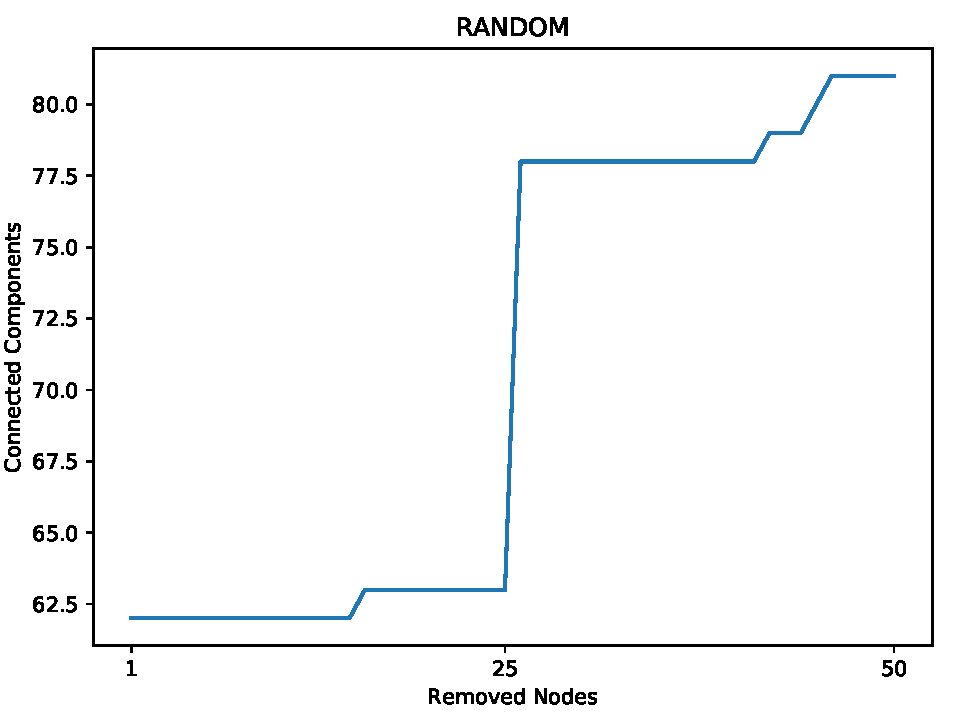
\includegraphics{images/robustness/test_cc_on_random.pdf}
                }
                \caption{}
                \label{test_cc_on_random}
            \end{subfigure}
            \begin{subfigure}{0.45\textwidth}
                \resizebox{\textwidth}{!}{
                    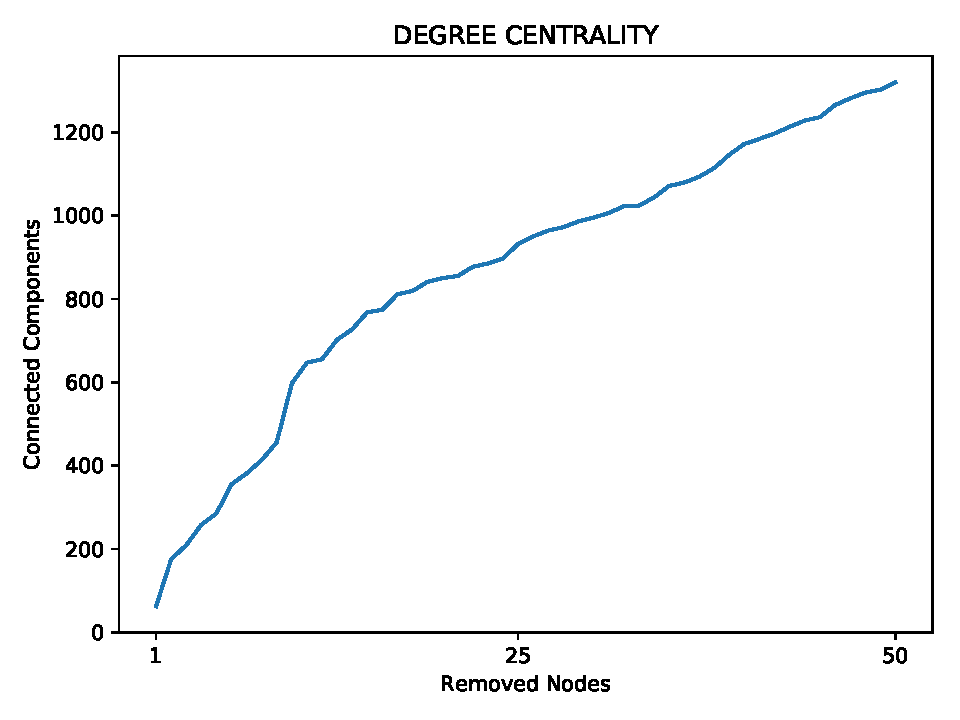
\includegraphics{images/robustness/test_cc_on_degree_centrality.pdf}
                }
                \caption{}
                \label{test_cc_on_degree_centrality}
            \end{subfigure}
            \caption{In Figure \ref{test_cc_on_random} we can see the fragmentation of the connected components
            during the remotion based on a randomic choice, while in Figure \ref{test_cc_on_degree_centrality} we
            can see the same fragmentation, but this time based on decreasing degree centraility.}
            \label{test_cc}
        \end{figure}

        As we can see, for the randomic choice of the nodes to be removed, the structure of the network is barely
        altered. After the random remotion of $50$ nodes, the original $62$ connected components became slightly
        more than $80$. For the remotion of the nodes based on decreasing degree centrality there is, as expected,
        a different situation. This kind of criterion guarantees that the original structure of the network is
        broken apart more easily, because the original network's hubs are removed one by one in decreasing order.
    % section simulation_of_an_attack (end)
    \section{Simulation of a Failure Propagation Model} % (fold)
    \label{sec:simulation_of_a_failure_propagation_model}
        To test more the robustness of our network, we've written the code in order to implement (and test) the
        \textbf{Failure Propagation Model}, as described in \cite{network_science}. In Figure \ref{fail_prop_model}
        you can see some iterations of the model in which we used different values for the $\varphi$ parameter.

        \begin{figure}[H]
            \centering
            \begin{subfigure}{0.50\textwidth}
                \resizebox{\textwidth}{!}{
                    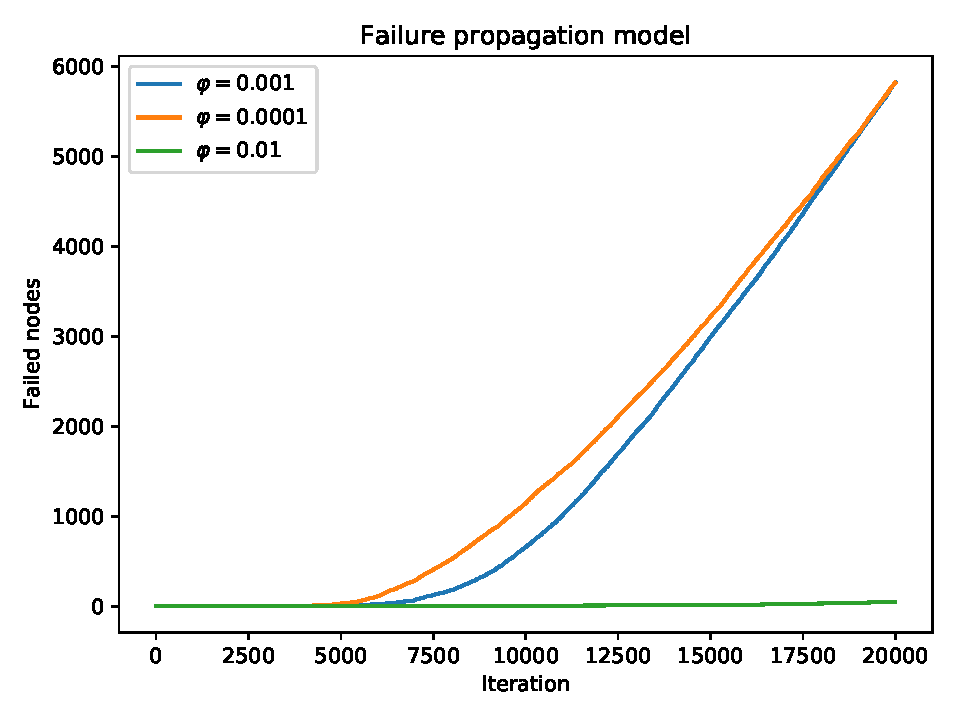
\includegraphics{images/robustness/failure_propagation_model.pdf}
                }
            \end{subfigure}
            \caption{The test for the Failure Propagation Model was conducted over $20000$ iterations.}
            \label{fail_prop_model}
        \end{figure}

        We can see that, as expected, the network doesn't accuse the failure propagation for $\varphi$ eguals to
        $0.01$, in which less than $30$ nodes failed. For the smaller values of $\varphi$ we can see that the
        situation is different, with a greater amount of nodes which fail over the iterations.
    % section simulation_of_a_failure_propagation_model (end)
% chapter network_robustness (end)
